\section{Обзор литературы}

Перед тем, как приступить непосредственно к разработке схемы цифрового осциллографа, следует ознакомиться с некоторыми необходимыми для понимания вопроса теоретическими сведениями.

\subsection{Принцип работы осциллографа}

Осциллограф - прибор, предназначенный для исследования амплитудных и временных параметров электрического сигнала. В отличие от амперметра и вольтметра, которые дают \textit{действующие значения} для переменного тока и напряжения, осциллограф служит для определения их \textit{мгновенных значений} \cite[с. 381]{esbe}.

\emph{Действующее значение переменного тока} - это величина постоянного тока, который за время, равное одному периоду переменного тока, произведёт такую же работу, что и рассматриваемый переменный ток \cite{yavorskiy}.

\emph{Мгновенное значение переменного тока} - его действительная величина в определенный момент времени;
именно посредством множества измерений мгновенного значения переменного тока осциллограф получает временное представление электрического сигнала.

Для понимания принципа работы цифрового осциллографа, рассмотрим рисунок
\ref{fig:inside}, на котором изображены его основные компоненты, а также упрощенное представление всего устройства.

\begin{figure}[H]
    \centering
    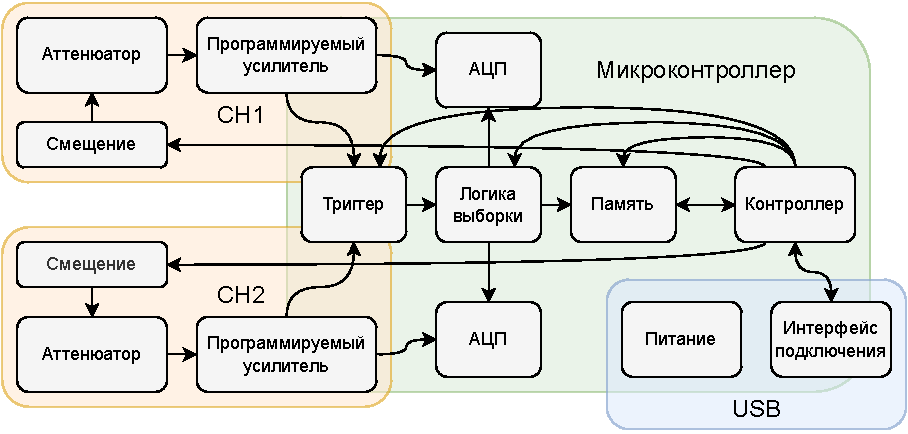
\includegraphics[width=0.95\linewidth]{inside.pdf}
    \caption{Упрощенное внутреннее представление двухканального цифрового осциллографа}
    \label{fig:inside}
\end{figure}

\emph{Аттенюатор} -- это пассивный компонент в высокочастотной технике, которое уменьшает амплитуду или мощность сигнала без существенного искажения его формы.

\emph{Операционный усилитель} --  это электронный усилитель напряжения с высоким коэффициентом усиления, имеющий дифференциальный вход, также называемый входом напряжения.

\emph{Аналого-цифровой преобразователь} -- это устройство, преобразующее входной аналоговый сигнал в цифровой сигнал.

\emph{Триггер (trigger, защелка)} -- это схема с несколькими устойчивыми состояниями; в данном случае под триггером понимается схема, имеющая вход и устанавливаемый порог срабатывания.

Принцип работы цифрового осциллографа состоит из нескольких последовательных действий:
\begin{enumerate}

    \item Входное напряжение проходит через усилитель вертикального отклонения с делителем. Таким образом обеспечивается дополнительное масштабирование сигнала.

    \item При помощи АЦП напряжение преображается в дискретную последовательность кодов - выполняется оцифровка сигнала.

    \item В кодах находят отображение мгновенные значения напряжения, после чего они записываются в оперативной памяти.

    \item Данные продолжают сохраняться в памяти до тех пор, пока на одной из выборок не происходит срабатывание триггера: после этого начинается передача данных по интерфейсу подключения.
\end{enumerate}

Стоит отметить, что \emph{сигнал смещения} используется для <<центрирования>> входного сигнала относительно нуля: это делается потому что последующие элементы цепи преобразования не могут работать с отрицательными значениями напряжения \cite{clamper}.

Как правило, изначально триггер работает в \emph{автоматическом режиме}, что позволяет получать развертку сигнала даже без срабатывания по определенному уровню, однако
режим срабатывания триггера можно изменить: например, можно указать срабатывание по возрастанию или спаду на определенном значении, что позволит получить осциллограмму тогда, когда форма сигнала достигнет указанных условий \cite{trigger}.

\subsection{Интерфейс USB}

\emph{USB (Universal Serial Bus, «Универсальная последовательная шина»)} -- последовательный интерфейс для подключения периферийных устройств к вычислительной технике \cite{usb}.

Интерфейс позволяет не только обмениваться данными, но и обеспечивать электропитание периферийного устройства. Сетевая архитектура позволяет подключать большое количество периферии даже к устройству с одним разъёмом USB.

В данном проекте в качестве интерфейса подключения к персональному компьютеру используется USB Type-A, изображение которого представлено на рисунке \ref{fig:usba}.

\begin{figure}[H]
    \centering
    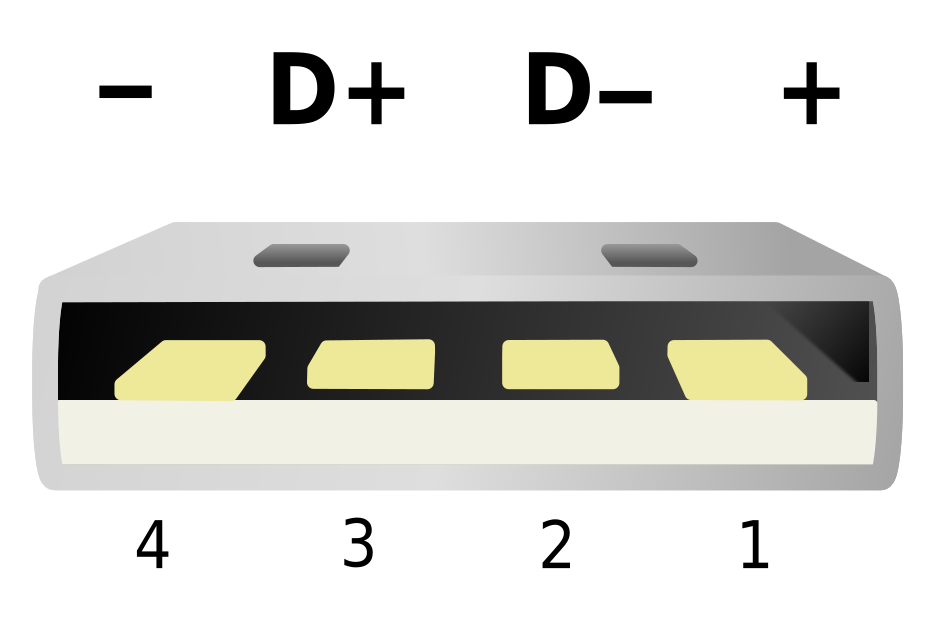
\includegraphics[width=0.5\linewidth]{images/USB.png}
    \caption{Стандартный коннектор USB Type-A}
    \label{fig:usba}
\end{figure}

В таблице \ref{tab:usba-pins} указана распиновка контактов коннектора с указанием их обозначения и описанием.

\begin{table}[H]
    \caption{Распиновка USB Type-A}
    \label{tab:usba-pins}
    \begin{tabular}{|l|l|l|}
        \hline
        Пин & Обозначение & Описание                                \\ \hline
        1   & $V_{BUS}$   & +5V (питание)                           \\ \hline
        2   & $D-$          & Data- (отрицательный сигнал данных)   \\ \hline
        3   & $D+$          & Data+ (положительный сигнал данных)   \\ \hline
        4   & $GND$         & Земля                                 \\ \hline
\end{tabular}
\end{table}